\documentclass{article}

\usepackage[romanian]{babel}
\usepackage[a4paper]{geometry}
\usepackage[hidelinks]{hyperref}
\usepackage[section]{placeins}

\usepackage{amsmath}
\usepackage{booktabs}
\usepackage{graphicx}
\usepackage{listings}
\usepackage{multirow}
\usepackage{pdflscape}

\graphicspath{{./images/}}

\title{{\huge ML}\\ Tema 2 --- Inteligență Artificială}
\author{Alexandru Sima (332CA)}

\begin{document}

\maketitle
\begin{abstract}
    Analiza a 2 seturi mari de date --- indici de calitate ai aerului și 
    informații despre popularitatea unor știri --- folosind tehnici de învățare
    automată, prelucrarea acestora în vederea antrenării unor modele de 
    clasificare. Clasificarea acestora folosind \textbf{Arbori de decizie}, 
    \textbf{Păduri aleatoare}, \textbf{Regresii logistică} și \textbf{Rețele 
    neurale adânci}. Comparații ale performanțelor modelelor.
\end{abstract}

\newpage
\tableofcontents

\newpage
\section{Poluarea aerului}
Primul set de date conține date despre diferiți parametri măsurați ai aerului,
în peste $20.000$ de orașe din întreaga lume. Prin antrenarea unui model de
învățare automată, se dorește clasificarea orașelor în funcție de gradul de 
riscuri pentru sănătate.

\subsection{Analiza datelor}
\subsubsection{Analiza valorică}
Setul de date conține $23.463$ de înregistrări, fiecare având 15 atribute, 
dintre care 7 numerice și 8 categorice (incluzând și atribul țintă 
\textit{AQI\_Category}).

Din statisticile obținute pentru atributele numerice la (\ref{fig:pol:num_attr}), 
observăm că numai \textit{Ozone\_Value} conține valori lipsă și că plajele de 
valori sunt destul de variate (spre exemplu, valorile \textit{AQI\_Value} se 
situează în principal în plaja de 40-80, pe când \textit{CO\_Value} are valori 
foarte apropiate de 0). Aceste fapte se observă și trasând \textit{boxplot}-ul
valorilor (\ref{fig:pol:num_boxplot}), de unde se poate observa mai clar 
"tendințele" outlierilori: deși în anumite cazuri (\textit{CO\_Value}, 
\textit{NO2\_Value}, \textit{SO2} într-o anumită măsură), valorile mari sunt în
mod flagrant eronate, în celelalte cazuri valorile sunt distribuite relativ 
unifom cu mult în afara plajei inter-cuartilă\footnote{
    \href{https://en.wikipedia.org/wiki/Interquartile_range}{IRQ --- 
    Interquartile Range}; plaja de valori dintre prima ($25\%$) și a treia 
    ($75\%$) cuartilă. Afișată în boxplot-uri printr-un segment.
}, ceea ce ar determina eliminarea a mult prea multe valori considerate outlier.
De aceea, se vor considera outlieri doar valorile care depășesc 
$1,5 \cdot \text{IQR}$, cu "cuartilele"\footnote{impropriu numite astfel} mult 
mai depărtate: $0,1$, respectiv $0,9$.

\begin{figure}[htb]
    \centering
    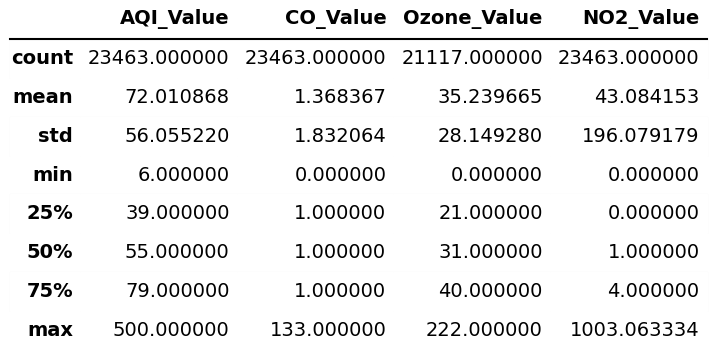
\includegraphics[scale=0.55]{air_pollution/analysis/numeric/table1.png}
    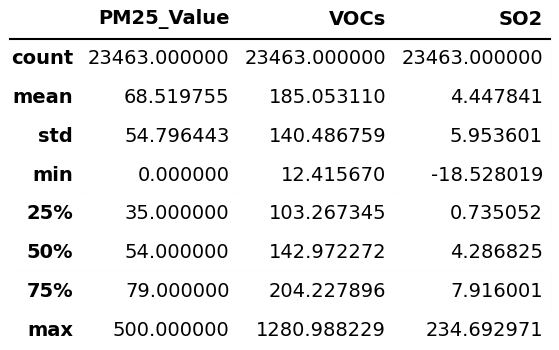
\includegraphics[scale=0.55]{air_pollution/analysis/numeric/table2.png}
    
    \caption{Statistici despre atributele numerice ale setului de date}
    \label{fig:pol:num_attr}
\end{figure}

\begin{figure}[htb]
    \centering
    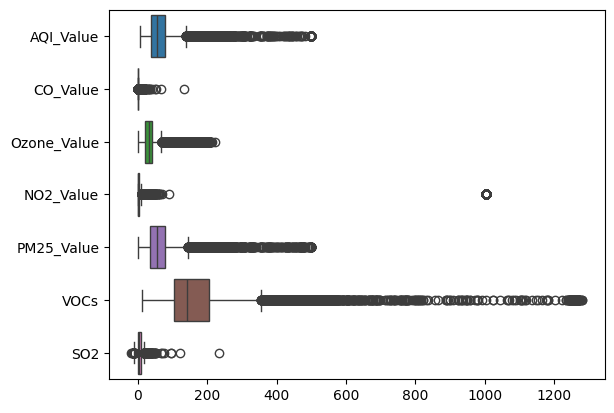
\includegraphics[scale=0.7]{air_pollution/analysis/numeric/boxplot.png}
    \caption{Boxplot pentru atributele numerice ale setului de date}
    \label{fig:pol:num_boxplot}
\end{figure}

Analizând atributele categorice la (\ref{fig:pol:cat_attr}), se observă că 
există valori lipsă pentru \textit{Ozone\_Category} și \textit{City}, deși
atributul din urmă poate fi complet eliminat, fiecare coloană reprezentând câte
un oraș diferit, acesta neputând fi folosit pentru niciun fel de corelație. Din
histogramele atributelor realizate la (\ref{fig:pol:cat_target} și
\ref{fig:pol:cat_hists}), se observă că valorile atributelor nu sunt distribuite
uniform, inclusiv în cazul \textbf{AQI\_Category} (atribut țintă), ceea ce face
clasificarea mai dificilă.

\begin{figure}[htb]
    \centering
    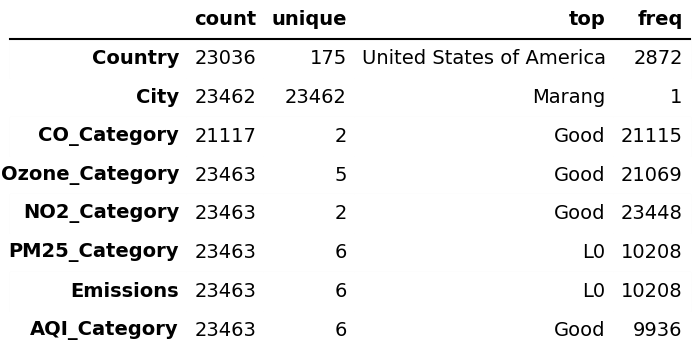
\includegraphics[scale=0.7]{air_pollution/analysis/categorical/table.png}
    \caption{Statistici despre atributele categorice ale setului de date}
    \label{fig:pol:cat_attr}
\end{figure}

\begin{figure}[htb]
    \centering
    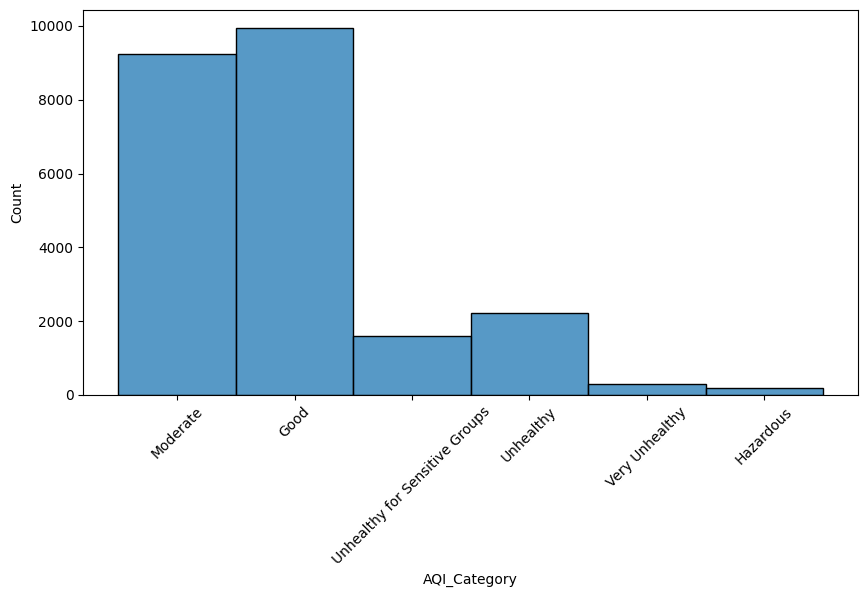
\includegraphics[scale=0.33]{air_pollution/analysis/categorical/target.png}
    \caption{Histogramă pentru atributul țintă al setului de date}
    \label{fig:pol:cat_target}
\end{figure}

\begin{figure}[htb]
    \centering
    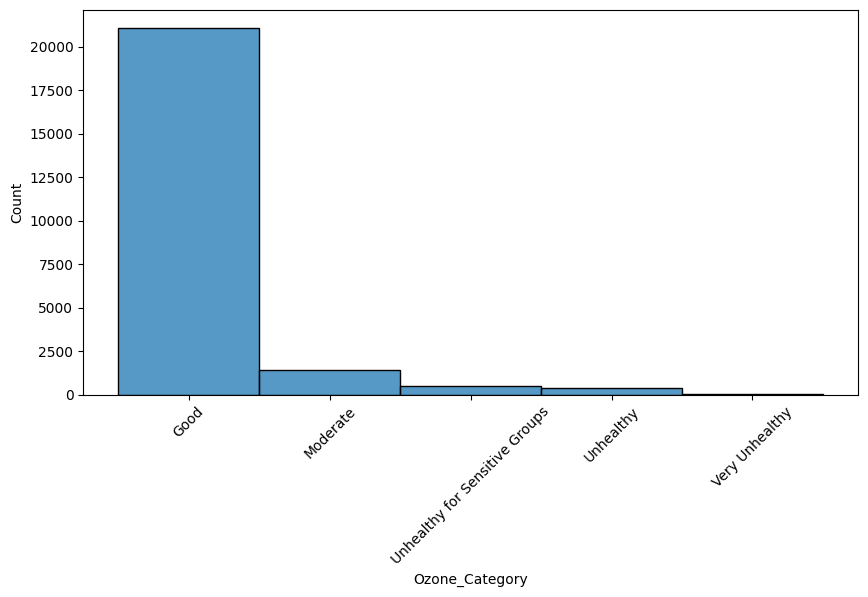
\includegraphics[scale=0.33]{air_pollution/analysis/categorical/o3.png}
    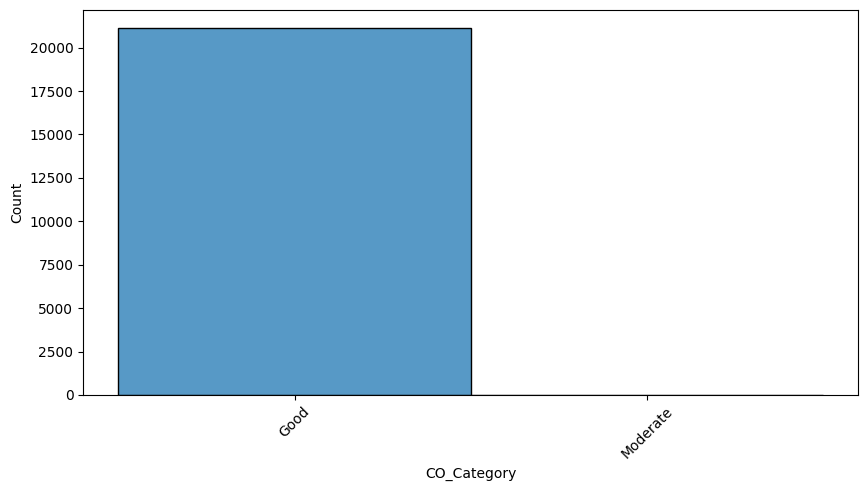
\includegraphics[scale=0.33]{air_pollution/analysis/categorical/co.png}
    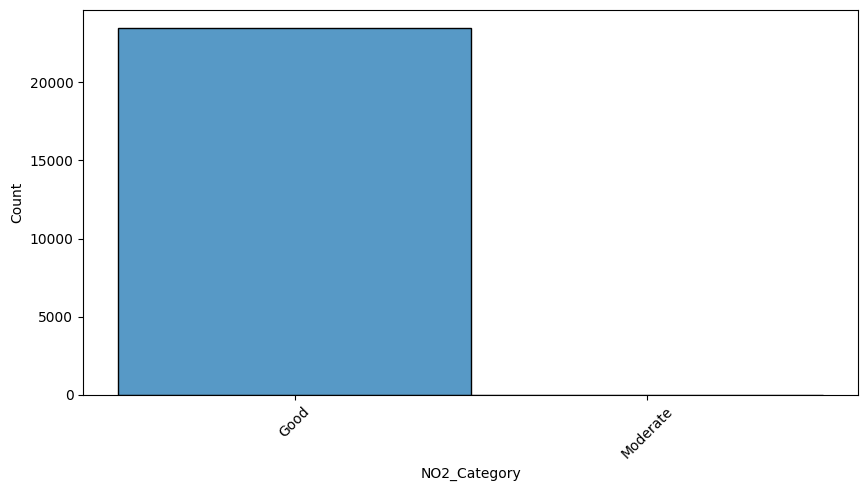
\includegraphics[scale=0.33]{air_pollution/analysis/categorical/no2.png}
    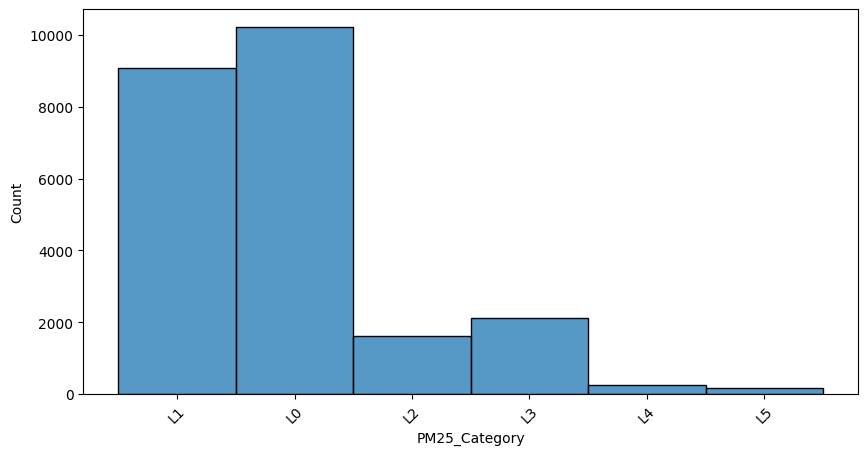
\includegraphics[scale=0.33]{air_pollution/analysis/categorical/pm25.png}
    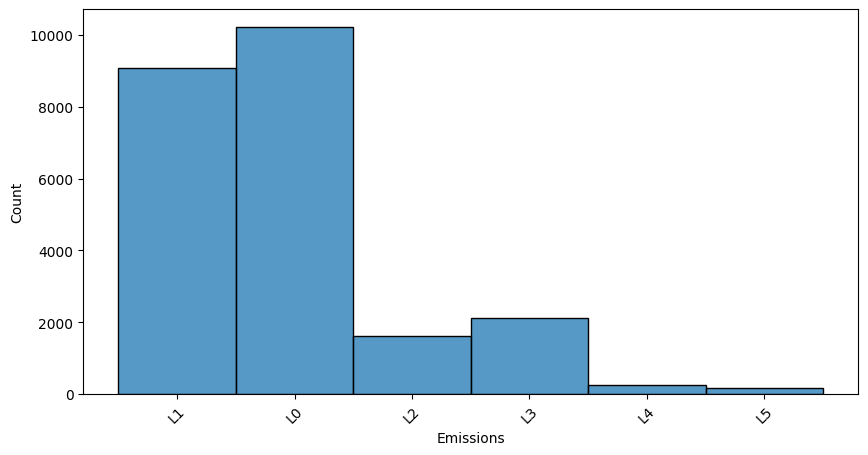
\includegraphics[scale=0.33]{air_pollution/analysis/categorical/emissions.png}
    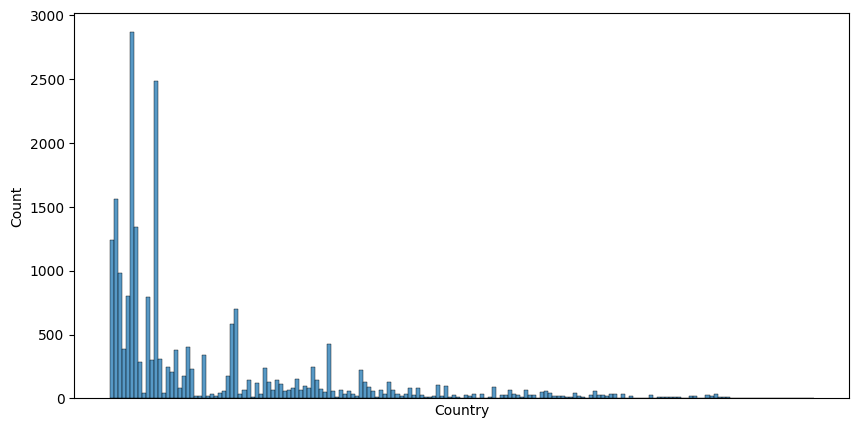
\includegraphics[scale=0.33]{air_pollution/analysis/categorical/country.png}
    \caption{Histograme pentru atributele categorice ale setului de date . 
    \textit{City} este ignorat din motivele enunțate anterior.}
    \label{fig:pol:cat_hists}
\end{figure}

\subsubsection{Analiza corelației atributelor}\label{sec:pol:corr}
Aplicând testul Pearson pentru a determina corelația liniară dintre atributele 
numerice, se obține matricea din (\ref{fig:pol:corr}). Se poate presupune
astfel că atributele \textit{AQI\_Value}, \textit{PM25\_Value} și \textit{VOCs}
sunt foarte puternic corelate între ele, având coeficientul de corelație 
$\geq 0.98$ și că atributul \textit{NO2\_Value} nu este corelat cu niciun altul, 
ceea ce ar putea indica lipsa de relevanță a acestui atribut în determinarea 
calității aerului. Într-adevăr, primele 3 atribute sunt puternic corelate, acest 
fapt observându-se trasând graficele valorilor (\ref{fig:pol:corr_graphs}). 
Testul Pearson oferă însă doar informații despre corelația liniară, astfel că, 
aplicând testul Spearman, se obține matricea din (\ref{fig:corr_spearman}), care
arată existența unor corelații între \textit{NO2\_Value} și alți parametri, 
fiind deci, până la urmă, relevant.

\begin{figure}[htb]
    \centering
    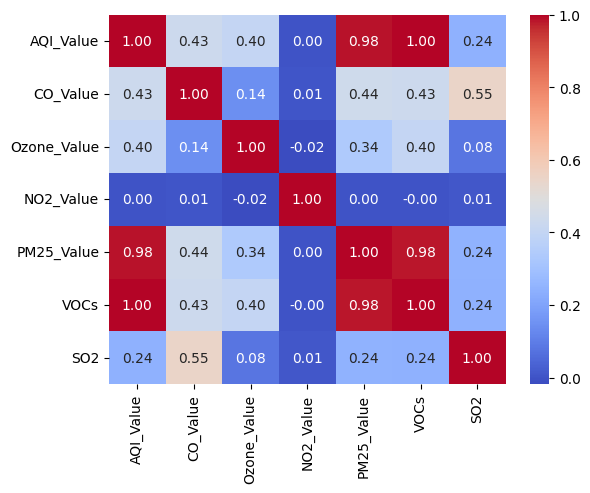
\includegraphics[scale=0.6]{air_pollution/analysis/correlation/matrix.png}
    \caption{Corelația dintre atributele setului de date, folosind coeficientul 
    Pearson}
    \label{fig:pol:corr}
\end{figure}

\begin{figure}[htb]
    \centering
    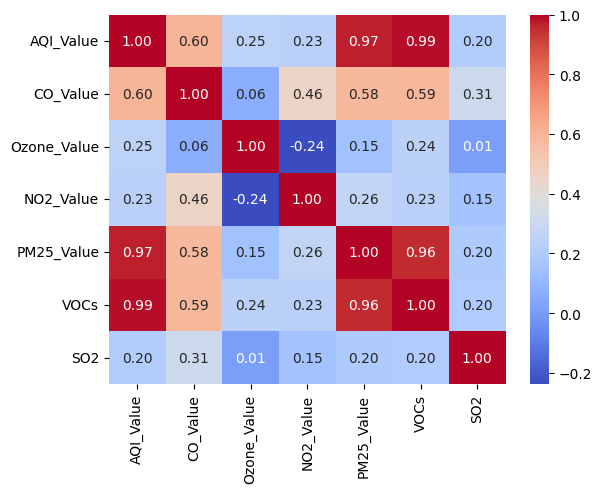
\includegraphics[scale=0.6]{air_pollution/analysis/correlation/matrix_spearman.png}
    \caption{Corelația dintre atributele setului de date, folosind coeficientul 
    Spearman}
    \label{fig:corr_spearman}
\end{figure}

\begin{figure}[htb]
    \centering
    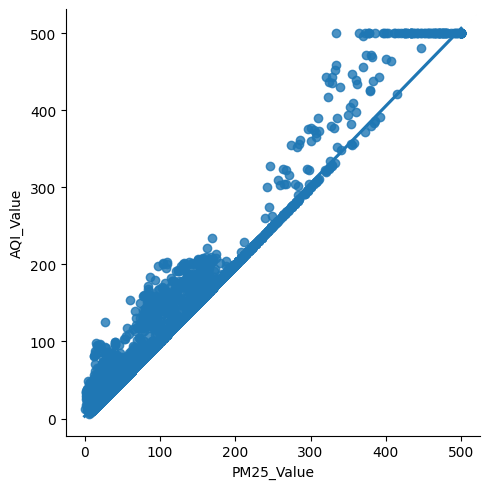
\includegraphics[scale=0.5]{air_pollution/analysis/correlation/aqi-pm25.png}
    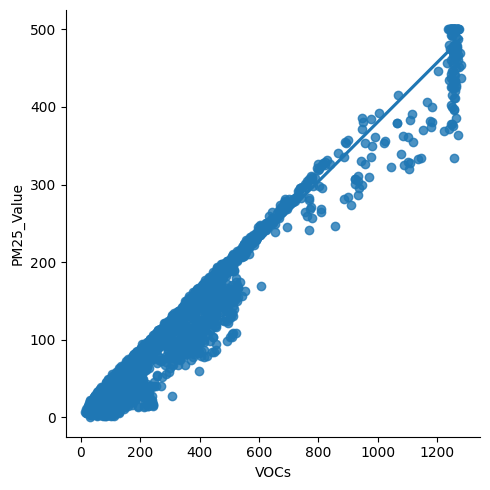
\includegraphics[scale=0.5]{air_pollution/analysis/correlation/pm25-vocs.png}
    \caption{Corelația liniară dintre \textit{AQI\_Value} și 
    \textit{PM25\_Value}, respectiv \textit{PM25\_Value} și \textit{VOCs}}
    \label{fig:pol:corr_graphs}
\end{figure}

În ceea ce privește corelația dintre atributele categorice, analiza este 
complicată de inegalitatea repartiției valorilor: deși testul $\chi^2$ de la 
(\ref{fig:pol:chi2}) indică o corelație puternică între toate atributele, mai
puțin \textit{City} cu oricare altul (evident) și perechile 
\textit{CO\_Category} - \textit{NO2\_Category} și \textit{Ozone\_Category} - 
\textit{PM25\_Category}, anumite corelații fiind doar aparente 
(\ref{fig:pol:cont}). Totuși, se remarcă o corelație pură: 
\textit{PM25\_Category} - \textit{Emissions} (\ref{fig:pol:cont_tot}), deci unul
dintre cele 2 atribute este superfluu. Am ales să elimin atributul 
\textit{PM25\_Category}.

\begin{figure}[htb]
    \centering
    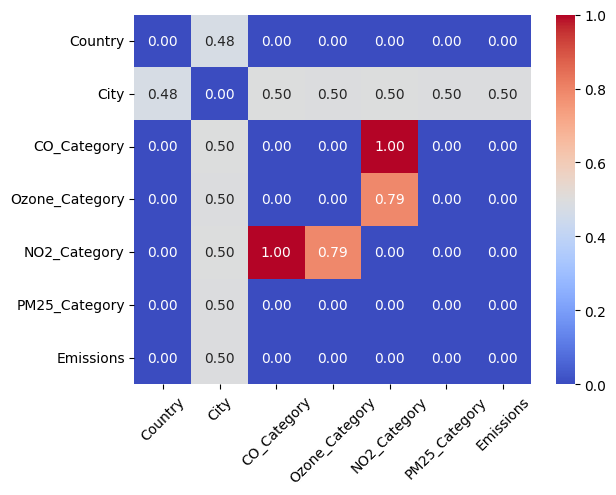
\includegraphics[scale=0.7]{air_pollution/analysis/correlation/chi2.png}
    \caption{Testul $\chi^2$ pentru atributele categorice ale setului de date}
    \label{fig:pol:chi2}
\end{figure}

\begin{figure}[htb]
    \centering
    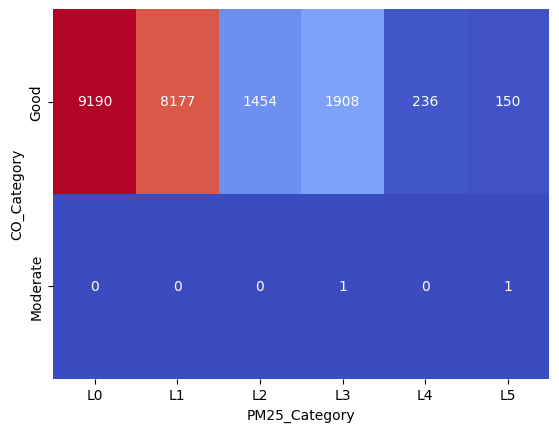
\includegraphics[scale=0.5]{air_pollution/analysis/correlation/co-pm25.png}
    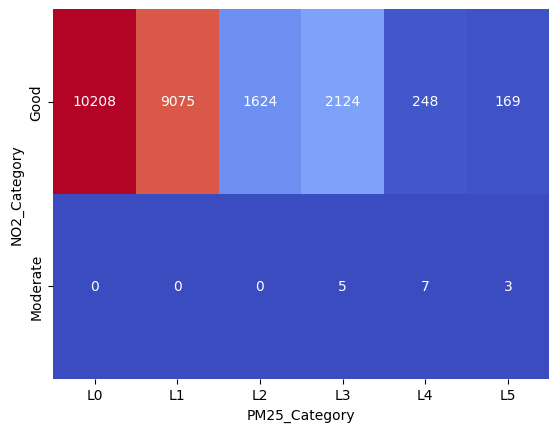
\includegraphics[scale=0.5]{air_pollution/analysis/correlation/no2-pm25.png}
    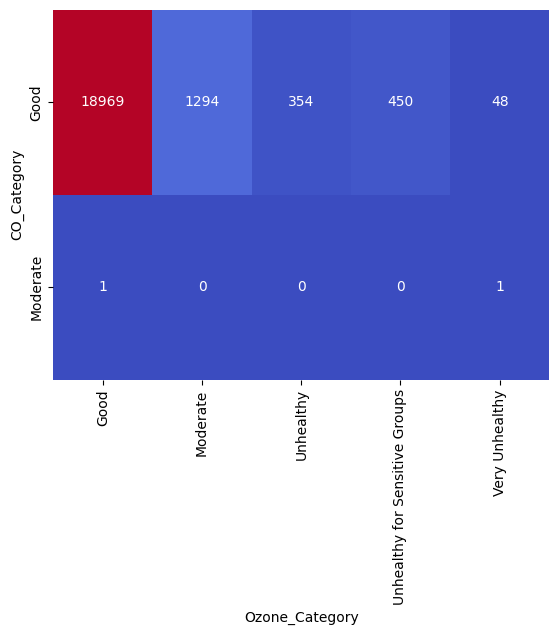
\includegraphics[scale=0.5]{air_pollution/analysis/correlation/co-o3.png}
    \caption{Câteva corelații puternice între atributele categorice ale setului 
    de date, datorate inegalității}
    \label{fig:pol:cont}
\end{figure}

\begin{figure}[htb]
    \centering
    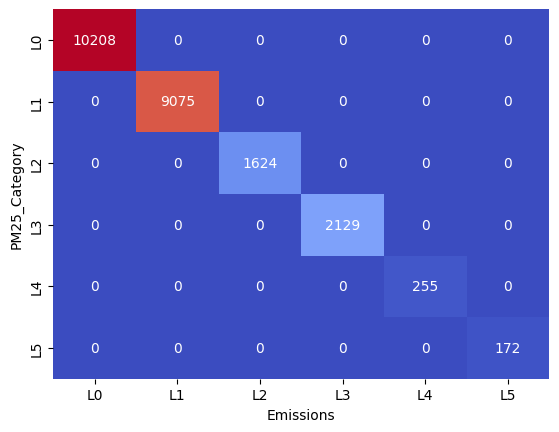
\includegraphics[scale=0.5]{air_pollution/analysis/correlation/pm25-emissions.png}
    \caption{Corelație totală între \textit{PM25\_Category} și 
    \textit{Emissions}}
    \label{fig:pol:cont_tot}
\end{figure}


\subsection{Preprocesarea datelor}\label{sec:pol:preproc}
Analizăm cunoștințele acumulate în urma analizei de mai sus a datelor, deducem 
că putem elimina anumite valori, pentru a îmbunătăți performanța modelului, fără
a afecta major acuratețea.

Transformarea datelor se face folosind pipeline-uri\footnote{
    \url{https://scikit-learn.org/stable/modules/generated/sklearn.pipeline.Pipeline}
}, pentru a fi consecventă --- aceeași transformare trebuie aplicată și datelor 
de antrenament, și celor de test. Singura excepție este eliminarea outlierilor,
care nu are sens decât pentru setul de antrenament.

\subsubsection{Eliminarea valorilor extreme}
Conform analizei de la (\ref{sec:pol:corr}), valorile au o dispersie foarte 
ridicată, deci noțiunea de outlier trebuie restricționată, pentru a nu pierde 
din acuratețe. 

\subsubsection{Imputarea valorilor lipsă}
Valorile lipsă, inclusiv cele eliminate la pasul anterior, sunt imputate 
folosind un \textit{SimpleImputer}\footnote{
    \url{https://scikit-learn.org/stable/modules/generated/sklearn.impute.SimpleImputer}
}, care completează valorile lipsă folosind mediana, respectiv moda (în cazul 
atributelor categorice). Imputarea multivariată (prin învățarea valorilor lipsă
din celelalte atribute), implementată prin \textit{IterativeImputer\footnote{
    \url{https://scikit-learn.org/stable/modules/generated/sklearn.impute.IterativeImputer}
}}, nu a dat rezultate mai bune, iar timpul de antrenare a crescut semnificativ.

\subsubsection{Eliminarea atributelor redundante}
Conform deciziilor de la (\ref{sec:pol:corr}), se elimină atributele 
\textit{AQI\_Value}, \textit{PM25\_Value} și \textit{PM25\_Category}, datorită 
corelațiilor și \textit{City}, datorită irelevanței.

\subsubsection{Normalizarea datelor}
Atributele numerice sunt normalizate folosind \textit{StandardScaler}\footnote{
    \url{https://scikit-learn.org/stable/modules/generated/sklearn.preprocessing.StandardScaler}
}, care le transformă astfel încât să aibă media 0 și deviația standard 1. Acest
pas este necesar pentru a asigura contribuția echitabilă a fiecărui atribut în 
regresia modeleleor de învățare. Normalizarea este importantă mai ales în cazul
regresiei logistice, deoarece valori mari (cu atât mai mult exponențiate) pot
eclipsa alți parametri.

\subsubsection{Codificarea atributelor categorice și a atributului țintă}
Inițial, am decis ca atributele categorice să fie codificate folosind \textit{OrdinalEncoder}\footnote{
    \url{https://scikit-learn.org/stable/modules/generated/sklearn.preprocessing.OrdinalEncoder}
}, care le transformă în numere întregi, fiecare valoare unică având un număr
corespunzător, dar, codificând în schimb prin \textit{OneHotEncoder}\footnote{
    \url{https://scikit-learn.org/stable/modules/generated/sklearn.preprocessing.OneHotEncoder}
}, se obțin rezultate mai bune, probabil existând o mai mare relevanță a unor 
valori specifice ale unei clase. 

\newpage
\subsection{Învățarea automată}

\subsubsection{Arbori de decizie}
Pentru a antrena un model de tip arbore de decizie, se folosește
\textit{DecisionTreeClassifier}\footnote{
    \url{https://scikit-learn.org/stable/modules/generated/sklearn.tree.DecisionTreeClassifier}
}, care îl construiește pe baza datelor de antrenament. Acesta este foarte 
performant, reușind, cu \underline{parametrizarea implicită}, o acuratețe de
$\approx 100\%$ pe setul de test, clasificând eronat, în medie, 3 intrări, 
conform matricei de confuzie de la (\ref{fig:pol:dt_conf}).

\begin{figure}[ht]
    \centering
    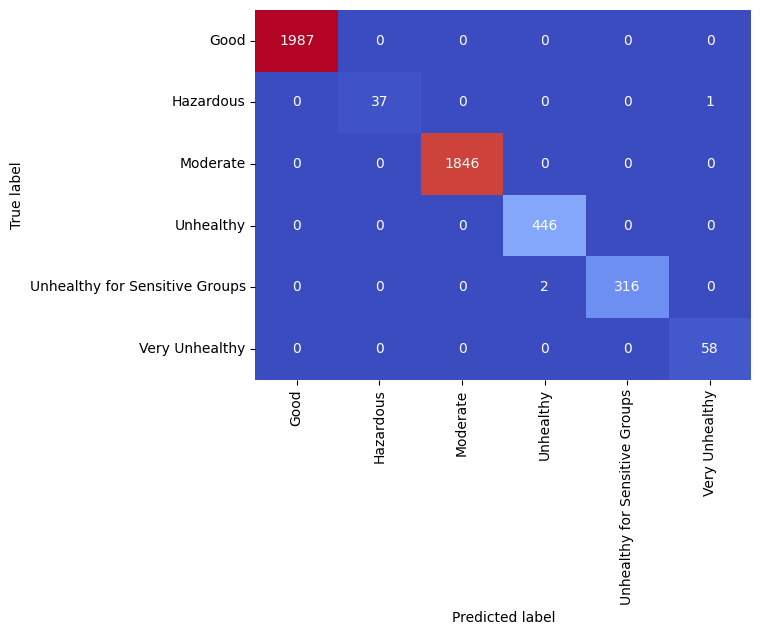
\includegraphics[scale=0.5]{air_pollution/learning/decision_conf.png}
    \caption{Matricea de confuzie a modelului de tip arbore de decizie}
    \label{fig:pol:dt_conf}
\end{figure}

\subsubsection{Păduri aleatoare}

Modelul de tip pădure aleatoare folosit este
\textit{RandomForestClassifier}\footnote{
    \url{https://scikit-learn.org/stable/modules/generated/sklearn.ensemble.RandomForestClassifier}
}, care reușește performanțe similare (conform (\ref{fig:pol:rf_conf})), 
având însă o performanță mai scăzută d.p.d.v. temporal ($\approx 1,6s$ vs 
$\approx 0,2s$).

\begin{figure}[ht]
    \centering
    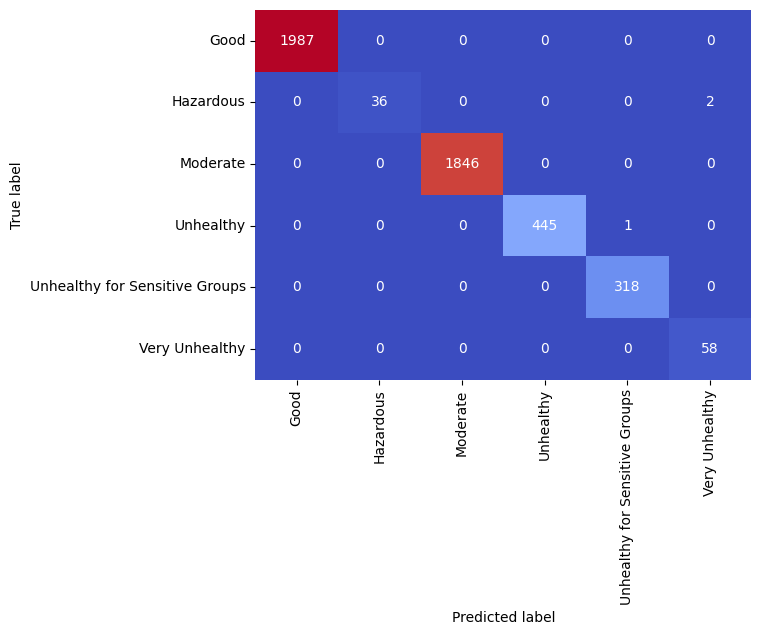
\includegraphics[scale=0.5]{air_pollution/learning/random_forest_conf.png}
    \caption{Matricea de confuzie a modelului de tip pădure aleatoare}
    \label{fig:pol:rf_conf}
\end{figure}

\subsubsection{Regresie logistică}\label{sec:pol:reg}
Modelul de regresie logistică este implementat manual. Cum regresia logistică
este folosită în mod obișnuit pentru clasificare binară, aceasta trebuie 
adaptată, realizând o clasificare de tip \textit{one-vs-rest}, antrenându-se 
câte un regresor pentru fiecare clasa, iar clasa prezisă fiind cea a cărei 
regresor întoarce o valoare maximă. Nu am implementat regularizare, datele fiind
în principiu normalizate, iar, prin testare, neobținându-se rezultate mai bune.
Pe setul de test, se obține o acuratețe de $\approx 87\%$ (conform 
(\ref{fig:pol:log_conf})).

\begin{figure}[htb]
    \centering
    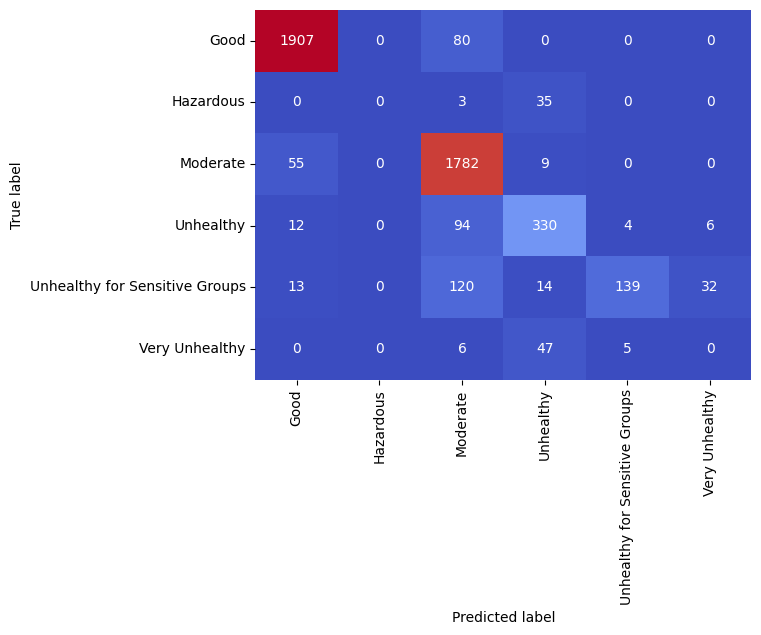
\includegraphics[scale=0.5]{air_pollution/learning/logistic_conf.png}
    \caption{Matricea de confuzie a modelului de regresie logistică}
    \label{fig:pol:log_conf}
\end{figure}

\subsubsection{Rețele neurale adânci}
Modelul de rețea neurală adâncă folosit este
\textit{MLPClassifier}\footnote{
    \url{https://scikit-learn.org/stable/modules/generated/sklearn.neural_network.MLPClassifier}
}, care reușește o acuratețe de $\approx 97\%$ (conform (\ref{fig:pol:nn_conf}))
pe setul de test, cu 2 straturi ascunse, fiecare a câte 64 de neuroni, restul 
parametrilor fiind cei impliciți.

\begin{figure}[htb]
    \centering
    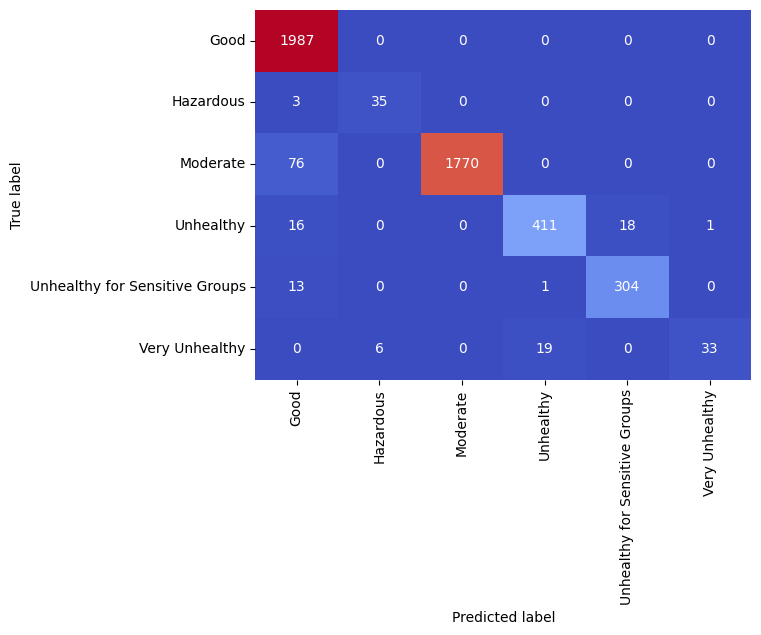
\includegraphics[scale=0.5]{air_pollution/learning/neural_network_conf.png}
    \caption{Matricea de confuzie a modelului de tip rețea neurală adâncă}
    \label{fig:pol:nn_conf}
\end{figure}

\begin{figure}[htb]
    \centering
    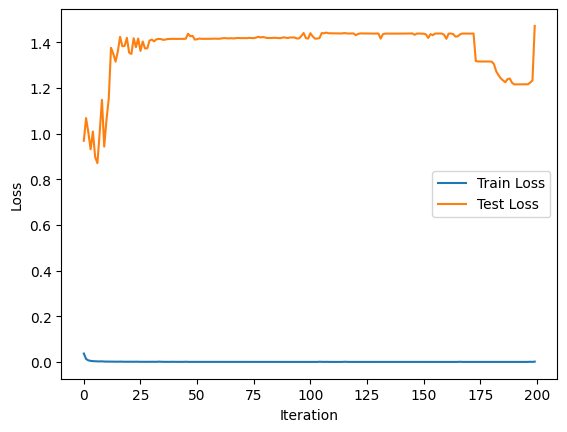
\includegraphics[scale=0.5]{air_pollution/learning/loss.png}
    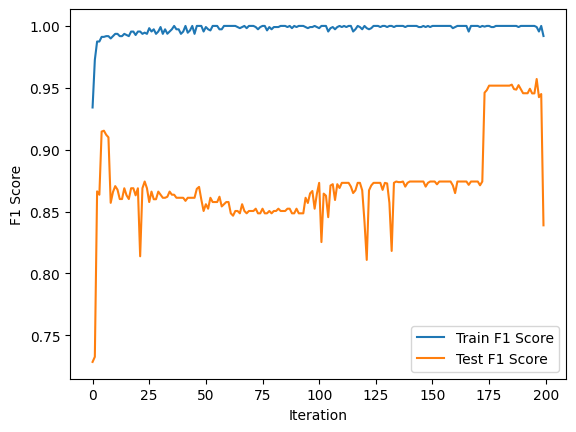
\includegraphics[scale=0.5]{air_pollution/learning/f1.png}
    \caption{Curbe de învățare și de acuratețe pentru rețea}
    \label{fig:pol:nn_loss}
\end{figure}

\subsection{Comparații}

Comparând performanțele modelelor, putem observa că arborii de decizie oferă 
cele mai bune rezultate, urmate de pădurile aleatoare, rețelele neurale și, în 
cele din urmă, regresia logistică. Se observă că clasele cel mai frecvent 
clasificate greșit sunt \textit{Hazardous} și \textit{Very Unhealthy}, care au 
și cel mai mic suport (sub 60 de valori fiecare). În particular, regresia 
logistică nu clasifică corect niciuna dintre aceste clase.

\begin{table}[htb]
\centering
\begin{tabular}{lcccc}
\toprule
\textbf{Class} & \textbf{Precision} & \textbf{Recall} & \textbf{F1-score} & \textbf{Support} \\
\midrule
Good                             & \textbf{1.00} & \textbf{1.00} & \textbf{1.00} & \textbf{1987} \\
Hazardous                        & \textbf{1.00} & \textbf{0.97} & \textbf{0.99} & 38   \\
Moderate                         & \textbf{1.00} & \textbf{1.00} & \textbf{1.00} & 1846 \\
Unhealthy                        & \textbf{1.00} & \textbf{1.00} & \textbf{1.00} & 446  \\
Unhealthy for Sensitive Groups  & \textbf{1.00} & \textbf{1.00} & \textbf{1.00} & 318  \\
Very Unhealthy                   & \textbf{0.98} & \textbf{1.00} & \textbf{0.99} & 58   \\
\midrule
\textbf{Accuracy}               &       &       & \textbf{1.00} & \textbf{4693} \\
\textbf{Macro avg}              & \textbf{1.00} & \textbf{1.00} & \textbf{1.00} & \textbf{4693} \\
\textbf{Weighted avg}           & \textbf{1.00} & \textbf{1.00} & \textbf{1.00} & \textbf{4693} \\
\end{tabular}
\caption{Raport de clasificare pentru arbori de decizie}
\end{table}

\begin{table}[htb]
\centering
\begin{tabular}{lcccc}
\hline
\textbf{Class} & \textbf{Precision} & \textbf{Recall} & \textbf{F1-score} & \textbf{Support} \\
\hline
Good                               & \textbf{1.00} & \textbf{1.00} & \textbf{1.00} & \textbf{1987} \\
Hazardous                          & \textbf{1.00} & 0.84 & 0.91 & 38   \\
Moderate                           & \textbf{1.00} & \textbf{1.00} & \textbf{1.00} & 1846 \\
Unhealthy                          & \textbf{1.00} & \textbf{1.00} & \textbf{1.00} & 446  \\
Unhealthy for Sensitive Groups     & \textbf{1.00} & \textbf{1.00} & \textbf{1.00} & 318  \\
Very Unhealthy                     & 0.90 & 0.98 & 0.94 & 58   \\
\hline
\textbf{Accuracy}                 &      &      & \textbf{1.00} & \textbf{4693} \\
\textbf{Macro avg}                & 0.98 & 0.97 & 0.98 & \textbf{4693} \\
\textbf{Weighted avg}             & \textbf{1.00} & \textbf{1.00} & \textbf{1.00} & \textbf{4693} \\
\hline
\end{tabular}
\caption{Raport de clasificare pentru păduri aleatoare}
\end{table}


\begin{table}[htb]
\centering
\begin{tabular}{lcccc}
\textbf{Class} & \textbf{Precision} & \textbf{Recall} & \textbf{F1-score} & \textbf{Support} \\
Good                             & 0.96 & 0.96 & 0.96 & \textbf{1987} \\
Hazardous                        & 0.00 & 0.00 & 0.00 & 38   \\
Moderate                         & 0.85 & 0.97 & 0.91 & 1846 \\
Unhealthy                        & 0.76 & 0.74 & 0.75 & 446  \\
Unhealthy for Sensitive Groups  & 0.94 & 0.44 & 0.60 & 318  \\
Very Unhealthy                   & 0.00 & 0.00 & 0.00 & 58   \\
\hline
\textbf{Accuracy}               &       &       & 0.89 & \textbf{4693} \\
\textbf{Macro avg}              & 0.59 & 0.52 & 0.54 & \textbf{4693} \\
\textbf{Weighted avg}           & 0.88 & 0.89 & 0.87 & \textbf{4693} \\
\end{tabular}
\caption{Raport de clasificare pentru regresia logistică}
\end{table}

\begin{table}[htb]
\centering
\begin{tabular}{lcccc}
\hline
\textbf{Class} & \textbf{Precision} & \textbf{Recall} & \textbf{F1-score} & \textbf{Support} \\
\hline
Good                               & \textbf{1.00} & 0.96 & 0.98 & \textbf{1987} \\
Hazardous                          & 0.16 & 0.95 & 0.28 & 38   \\
Moderate                           & \textbf{1.00} & 0.96 & 0.98 & 1846 \\
Unhealthy                          & 0.99 & 0.96 & 0.98 & 446  \\
Unhealthy for Sensitive Groups     & 0.99 & 0.96 & 0.98 & 318  \\
Very Unhealthy                     & 0.96 & 0.90 & 0.93 & 58   \\
\hline
\textbf{Accuracy}                 &      &      & 0.96 & \textbf{4693} \\
\textbf{Macro avg}                & 0.85 & 0.95 & 0.85 & \textbf{4693} \\
\textbf{Weighted avg}             & 0.99 & 0.96 & 0.97 & \textbf{4693} \\
\hline
\end{tabular}
\caption{Raport de clasificare pentru rețele neurale adânci}
\end{table}

\section{Popularitatea știrilor}
Al doilea set de date conține informații despre o selecție de aproape $40.000$ 
de articole știri de pe site-ul \url{https://www.mashable.com}, cuprinzând 
informații precum numărul de linkuri, de vizualizări, momentul publicării, 
categoria articolului și date despre cuvintele folosite. Ca și în cazul
setului de date anterior, se dorește clasificarea articolelor în funcție de
popularitatea acestora, aceasta cerință fiind mai dificilă, deoarece volumul de
date este mult mai mare.

\subsection{Analiza datelor}
\subsubsection{Analiza valorică}
Setul de date conține $39.644$ de înregistrări, fiecare având 64 de atribute. 47
dintre acestea sunt numerice, iar restul de sunt categorice (incluzând atributul
țintă \textit{popularity\_category}).

Analizând repartițiile atributelor numerice de la (\ref{fig:news:num_attr}),
(\ref{fig:news:num_attr2}), (\ref{fig:news:num_attr3}) și 
(\ref{fig:news:num_boxplot}), se observă că singura coloană cu valori lipsă 
este cea de \textit{content\_density} și, ca și în cazul anterior, că există
o distribuție foarte largă a valorilor, pe intervale de ordine de mărime foarte 
diferite: de exemplu, \textit{topic\_relevance} și \textit{*\_rate} sunt 
rapoarte (în intervalul $0-1$), pe când \textit{keyword\_best\_avg\_shares} este
de ordinul sutelor de mii. Având acestea în vedere, se vor considera outlierii 
ca în cazul setului de date precedent, apoi se va aplica o procedură de 
normalizare a datelor.

\begin{figure}[htb]
    \centering
    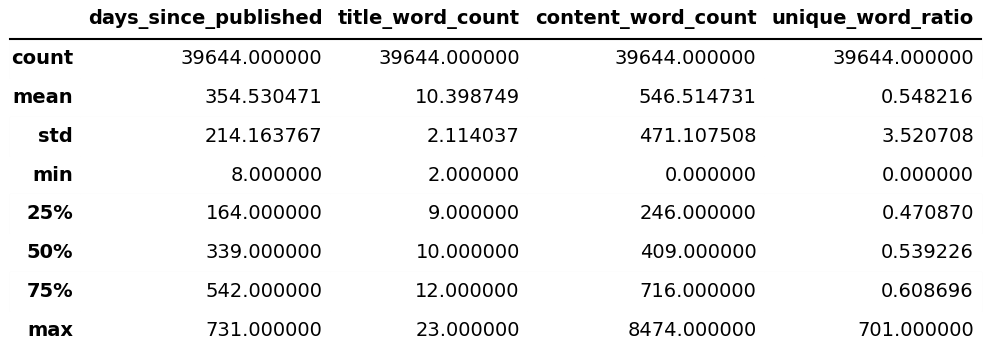
\includegraphics[scale=0.4]{news_popularity/analysis/numeric/table1.png}
    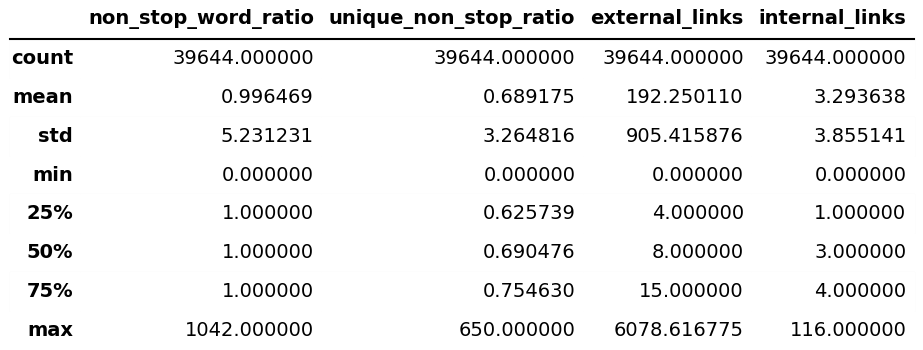
\includegraphics[scale=0.4]{news_popularity/analysis/numeric/table2.png}
    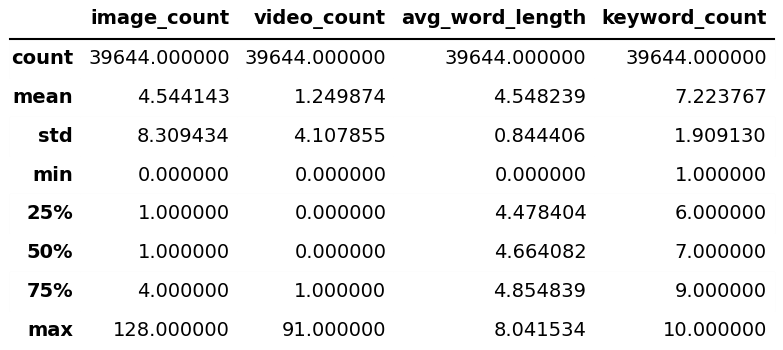
\includegraphics[scale=0.4]{news_popularity/analysis/numeric/table3.png}
    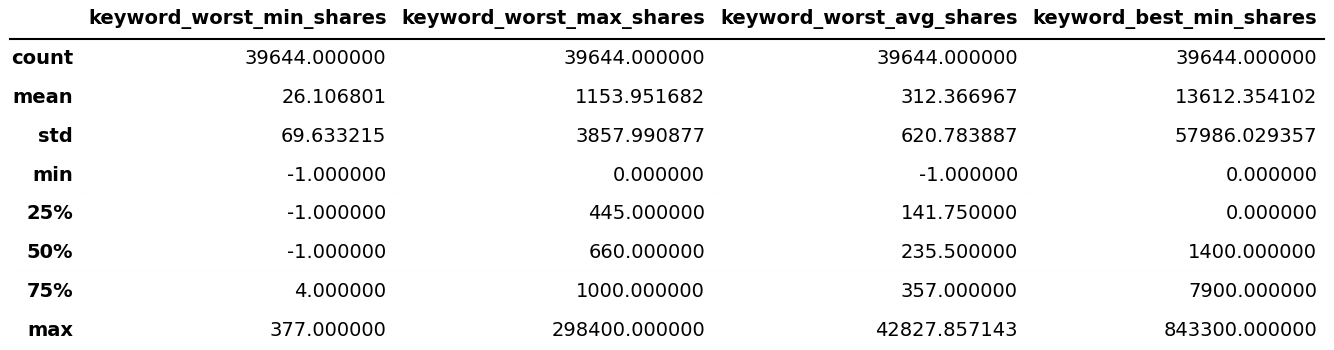
\includegraphics[scale=0.4]{news_popularity/analysis/numeric/table4.png}
    \caption{Statistici despre atributele numerice ale setului de date (1)}
    \label{fig:news:num_attr}
\end{figure}

\begin{figure}[htb]
    \centering
    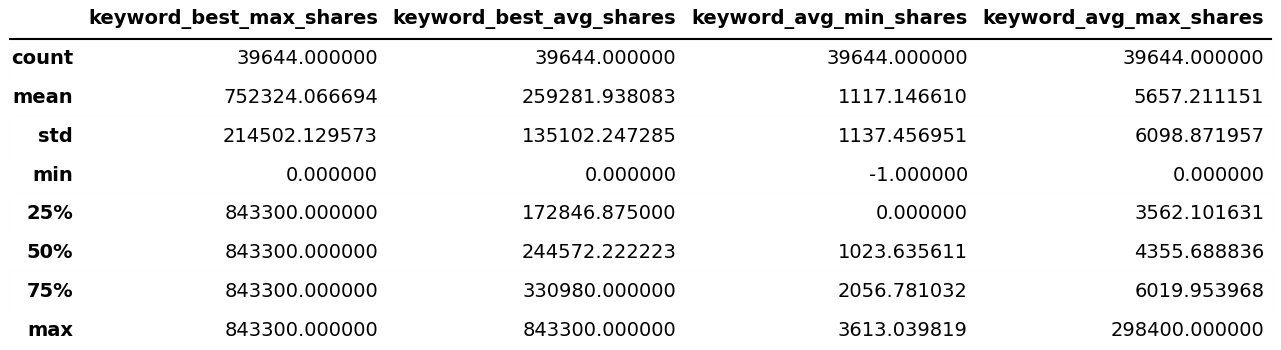
\includegraphics[scale=0.4]{news_popularity/analysis/numeric/table5.png}
    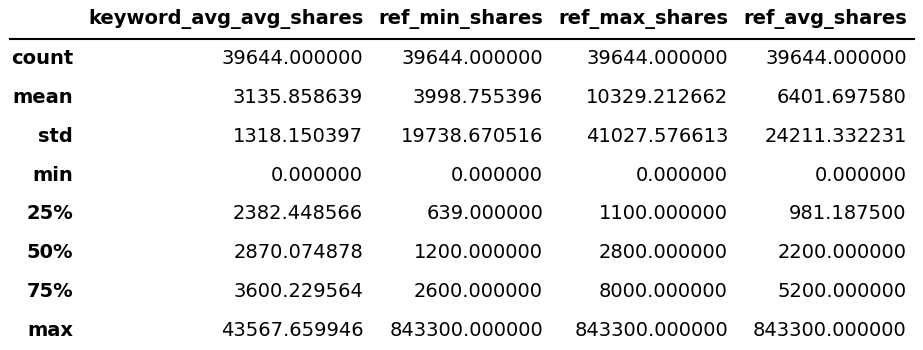
\includegraphics[scale=0.4]{news_popularity/analysis/numeric/table6.png}
    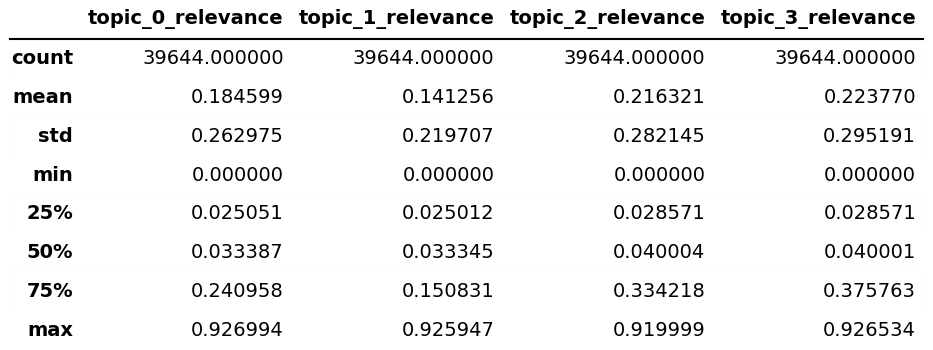
\includegraphics[scale=0.4]{news_popularity/analysis/numeric/table7.png}
    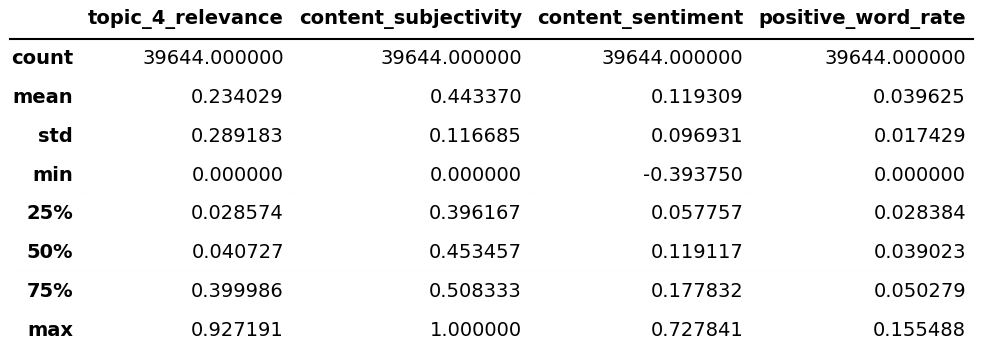
\includegraphics[scale=0.4]{news_popularity/analysis/numeric/table8.png}
    \caption{Statistici despre atributele numerice ale setului de date (2)}
    \label{fig:news:num_attr2}
\end{figure}

\begin{figure}[htb]
    \centering
    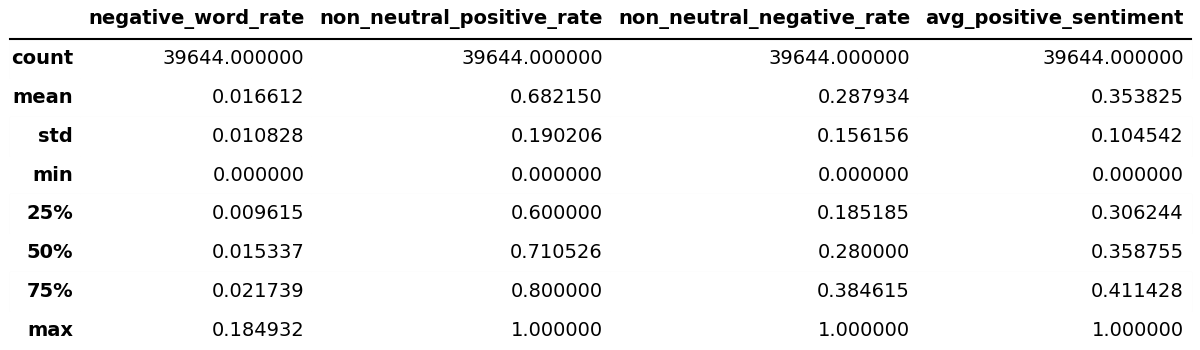
\includegraphics[scale=0.4]{news_popularity/analysis/numeric/table9.png}
    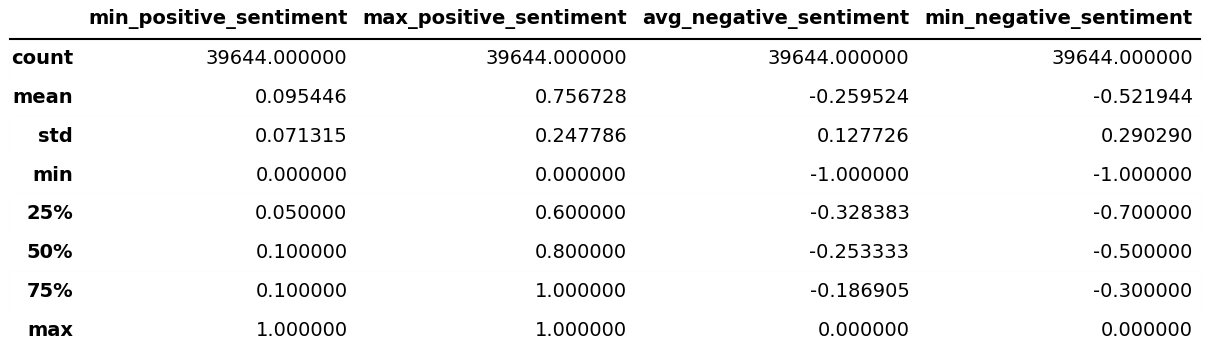
\includegraphics[scale=0.4]{news_popularity/analysis/numeric/table10.png}
    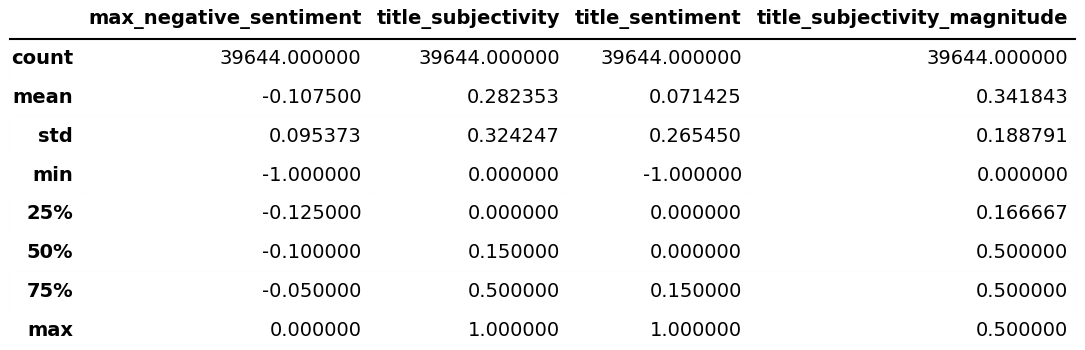
\includegraphics[scale=0.4]{news_popularity/analysis/numeric/table11.png}
    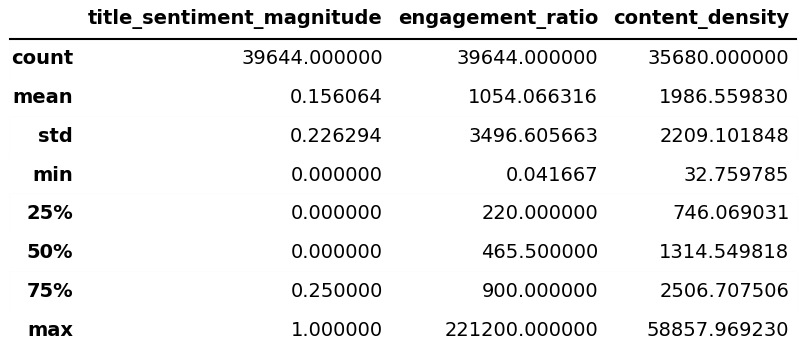
\includegraphics[scale=0.4]{news_popularity/analysis/numeric/table12.png}
    \caption{Statistici despre atributele numerice ale setului de date (3)}
    \label{fig:news:num_attr3}
\end{figure}

\begin{figure}[htb]
    \centering
    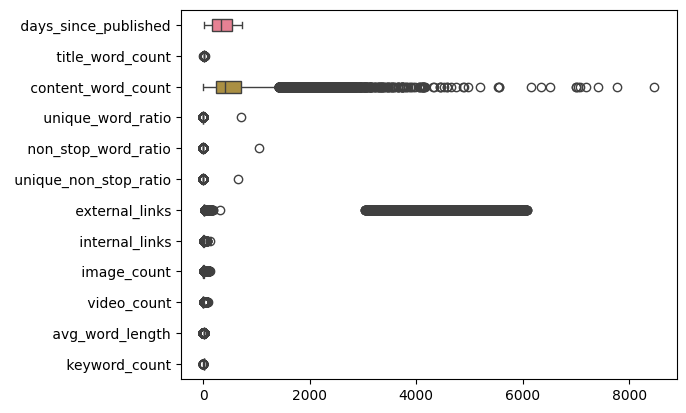
\includegraphics[scale=0.33]{news_popularity/analysis/numeric/boxplot1.png}
    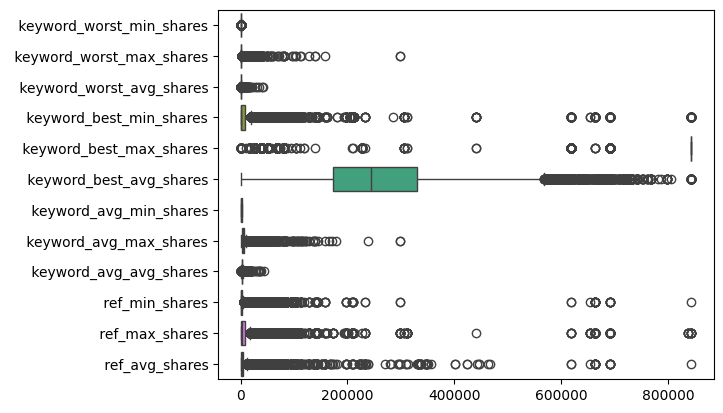
\includegraphics[scale=0.33]{news_popularity/analysis/numeric/boxplot2.png}
    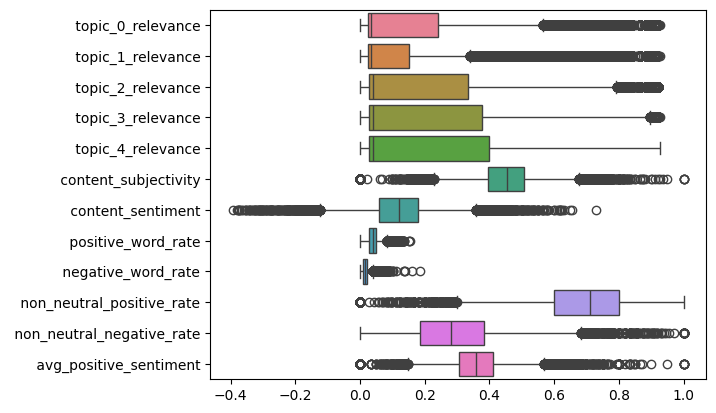
\includegraphics[scale=0.33]{news_popularity/analysis/numeric/boxplot3.png}
    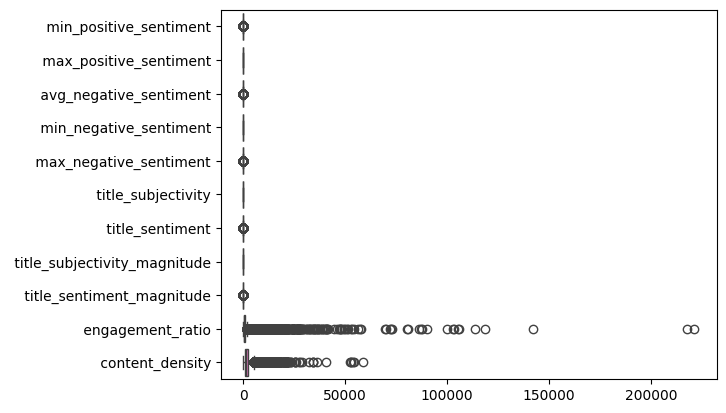
\includegraphics[scale=0.33]{news_popularity/analysis/numeric/boxplot4.png}
    \caption{Boxplot pentru atributele numerice ale setului de date}
    \label{fig:news:num_boxplot}
\end{figure}

În ceea ce privește atributele categorice, se observă din (\ref{fig:news:cat_attr}) că
există valori lipsă pentru \textit{channel\_lifestyle} și că, în afară de 
\textit{url} care are numai valori unice (precum \textit{City} în cazul 
poluării), toate atributele au doar 2 valori posiblie (de obicei "Yes" / "No").
De aceea, o codificare de tip one-hot nu își are rostul, adăugând câte un 
atribut în plus pentru fiecare valoare posibilă. Analizând histogramele de la 
(\ref{fig:news:cat_target}), (\ref{fig:news:cat_hists}) și 
(\ref{fig:news:cat_hists2}), se observă, din nou, o distribuție inegală, 
inclusiv în cazul atributului țintă \textbf{popularity\_category}, fiind totuși
mai uniformă decât în cazul setului de date precedent.  

\begin{figure}[htb]
    \centering
    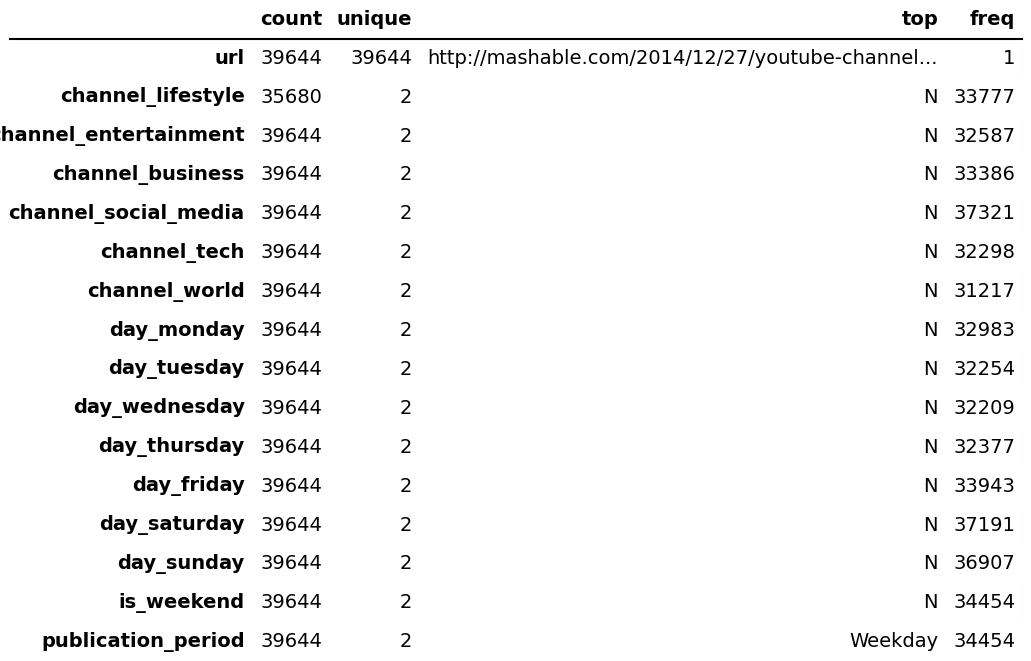
\includegraphics[scale=0.5]{news_popularity/analysis/categorical/table.png}
    \caption{Statistici despre atributele categorice ale setului de date}
    \label{fig:news:cat_attr}
\end{figure}

\begin{figure}[htb]
    \centering
    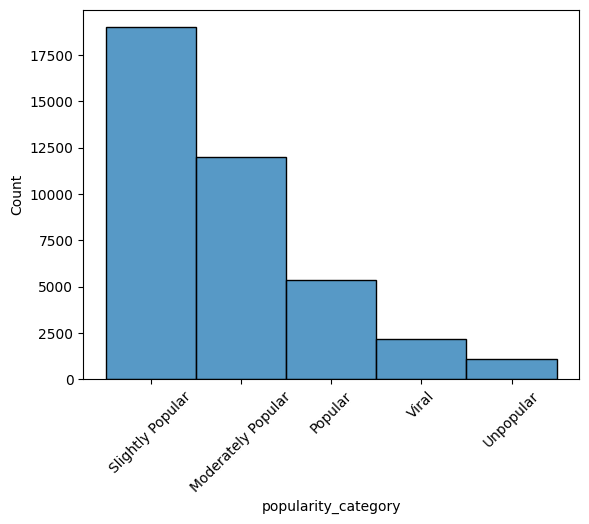
\includegraphics[scale=0.5]{news_popularity/analysis/categorical/target.png}
    \caption{Statistici despre atributul țintă al setului de date}
    \label{fig:news:cat_target}
\end{figure}

\begin{figure}[htb]
    \centering
    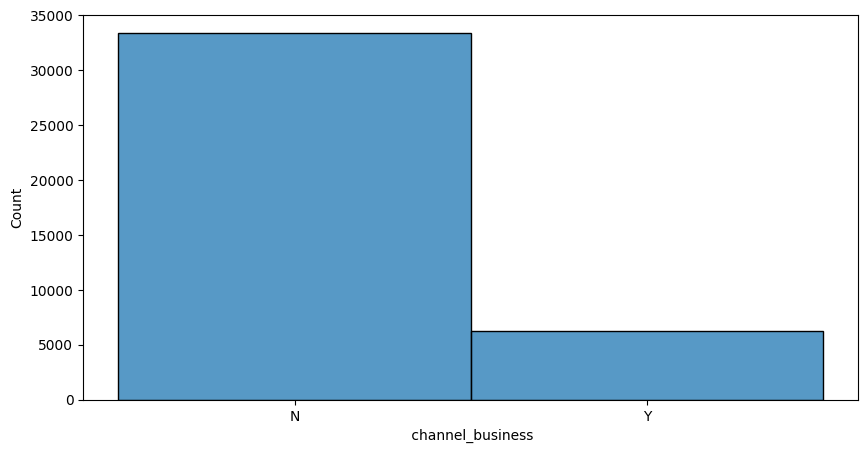
\includegraphics[scale=0.33]{news_popularity/analysis/categorical/channel_business.png}
    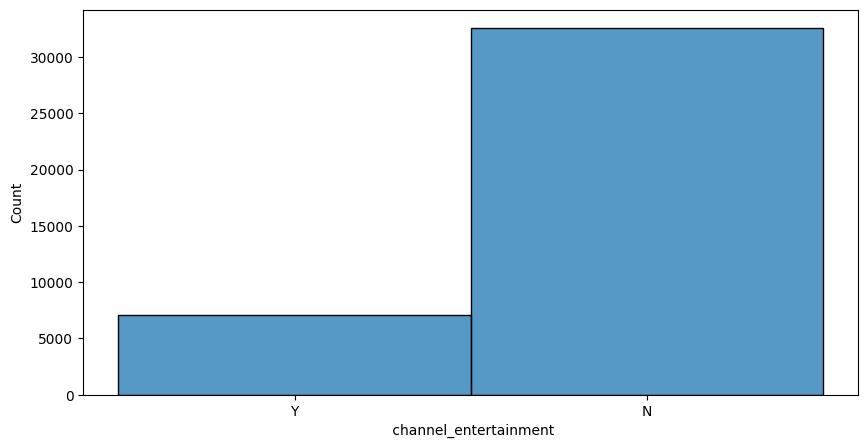
\includegraphics[scale=0.33]{news_popularity/analysis/categorical/channel_entertainment.png}
    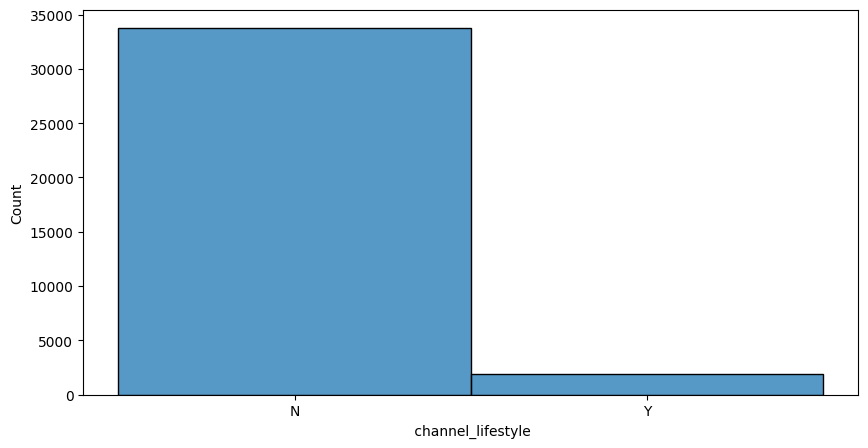
\includegraphics[scale=0.33]{news_popularity/analysis/categorical/channel_lifestyle.png}
    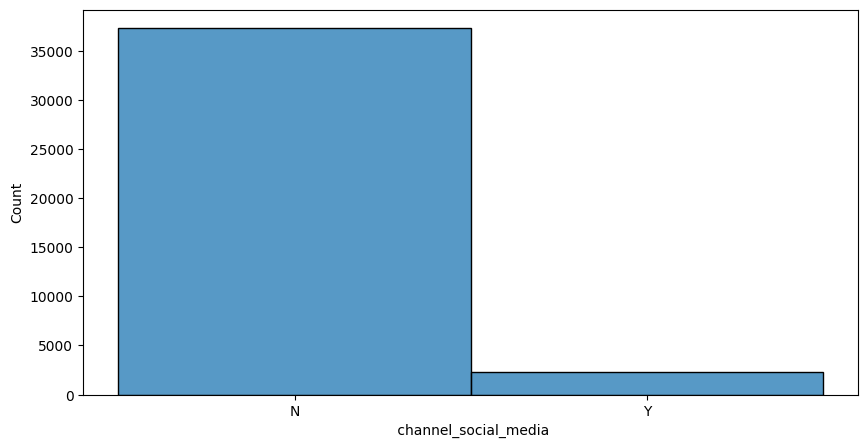
\includegraphics[scale=0.33]{news_popularity/analysis/categorical/channel_social_media.png}
    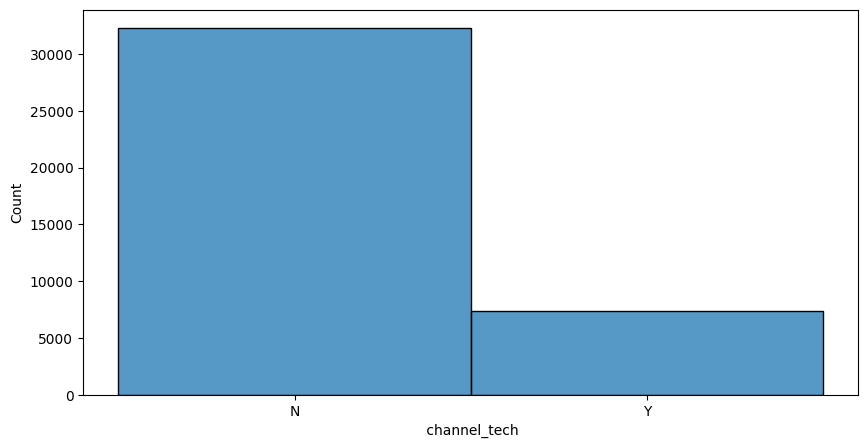
\includegraphics[scale=0.33]{news_popularity/analysis/categorical/channel_tech.png}
    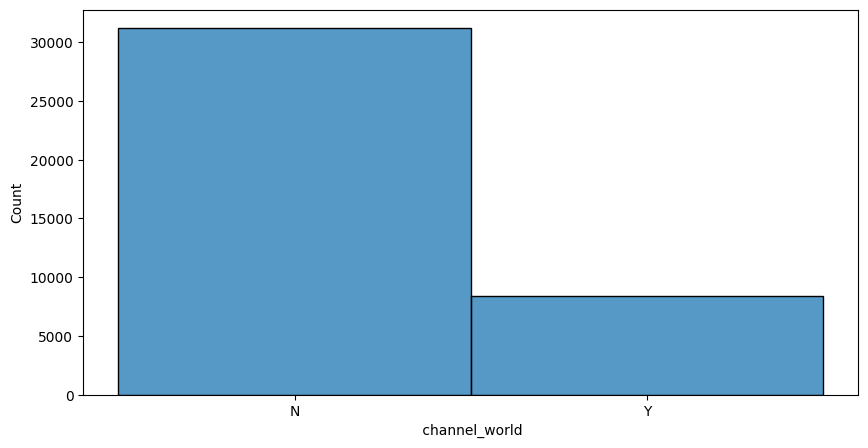
\includegraphics[scale=0.33]{news_popularity/analysis/categorical/channel_world.png}
    \includegraphics[scale=0.33]{news_popularity/analysis/categorical/day_monday.png}
    \includegraphics[scale=0.33]{news_popularity/analysis/categorical/day_tuesday.png}
   \caption{Histograme pentru atributele categorice ale setului de date 
    (incluzând atributul țintă). \textit{url} este ignorat. (1)}
    \label{fig:news:cat_hists}
\end{figure}

\begin{figure}[htb]
    \centering
    \includegraphics[scale=0.33]{news_popularity/analysis/categorical/day_wednesday.png}
    \includegraphics[scale=0.33]{news_popularity/analysis/categorical/day_thursday.png}
    \includegraphics[scale=0.33]{news_popularity/analysis/categorical/day_friday.png}
    \includegraphics[scale=0.33]{news_popularity/analysis/categorical/day_saturday.png}
    \includegraphics[scale=0.33]{news_popularity/analysis/categorical/day_sunday.png}
    \includegraphics[scale=0.33]{news_popularity/analysis/categorical/is_weekend.png}
    \includegraphics[scale=0.33]{news_popularity/analysis/categorical/publication_period.png}
    \caption{Histograme pentru atributele categorice ale setului de date (2)}
    \label{fig:news:cat_hists2}
\end{figure}
 

\subsubsection{Analiza corelației atributelor}

Analizând corelația dintre atributele numerice folosind coeficientul Pearson,
se obține matricea din (\ref{fig:news:corr}). Trasând graficele de corelație 
dintre atributele cu un indice ridicat ($|p| \geq 0.9$), se observă în 
(\ref{fig:news:invalid_corr_graphs}) că există niște corelații date în mod 
eronat de outlieri: \textit{non\_stop\_word\_ratio} - 
\textit{unique\_non\_stop\_word\_ratio} și \textit{unique\_word\_ratio} - 
\textit{non\_stop\_word\_ratio}. În schimb, corelații liniare evidente relevă 
din (\ref{fig:news:corr_graphs}) între perechile 
\textit{keyword\_worst\_max\_shares} - \textit{keyword\_worst\_avg\_shares} și 
\textit{content\_word\_count} - \textit{content\_density}. Am ales să elimin
\textit{keyword\_worst\_avg\_shares} și \textit{content\_word\_count}.

\begin{figure}[htb]
    \centering
    \includegraphics[scale=0.6]{news_popularity/analysis/correlation/matrix.png}
    \caption{Corelația dintre atributele numerice ale setului de date, folosind 
    coeficientul Pearson}
    \label{fig:news:corr}
\end{figure}

\begin{figure}[htb]
    \centering
    \includegraphics[scale=0.5]{news_popularity/analysis/correlation/nonstop-unique.png}
    \includegraphics[scale=0.5]{news_popularity/analysis/correlation/unique-nonstop.png}
    \caption{Corelații eronate între atributele numerice ale setului de date
    datorate outlierilor}
    \label{fig:news:invalid_corr_graphs}
\end{figure}

\begin{figure}[htb]
    \centering
    \includegraphics[scale=0.5]{news_popularity/analysis/correlation/max-avg.png}
    \includegraphics[scale=0.5]{news_popularity/analysis/correlation/count-density.png}
    \caption{Corelații puternice între atributele numerice ale setului de date}
    \label{fig:news:corr_graphs}
\end{figure}

În ceea ce privește corelația între atributele categorice (calculată la 
(\ref{fig:news:chi2})), aceasta este logică din moment ce majoritatea provin
dintr-o codificare one-hot a unor atribute (de exemplu, \textit{day\_monday} 
adevărat determină implicit ca toate celelalte zile ale săptămânii să fie false). 
Nu are sens să eliminăm aceste atribute. Totuși, există o redundanță evidentă:
\textit{day\_*} vs \textit{is\_weekend}. În funcție de scop, se poate alege 
păstrarea anumitor atribute. În cazul acesta, am ales să elimin 
\textit{is\_weekend}, păstrând mai multe informații (ce zi este, nu doar dacă
este weekend sau nu) în speranța că se va atinge o acuratețe mai mare.

\begin{figure}[htb]
    \centering
    \includegraphics[scale=0.7]{news_popularity/analysis/correlation/chi2.png}
    \caption{Testul $\chi^2$ pentru atributele categorice ale setului de date}
    \label{fig:news:chi2}
\end{figure}

\subsection{Preprocesarea datelor}
Modul de preprocesare a datelor este similar cu cel descris la 
(\ref{sec:pol:preproc}). Singurele diferențe sunt selectarea atributelor 
relevante și codificarea atributelor categorice.

\subsubsection{Eliminarea atributelor redundante}
Conform rezultatelor de mai sus, se elimină atributele \textit{url}, 
\textit{is\_weekend}, \textit{keyword\_worst\_avg\_shares} și 
\textit{content\_word\_count}.

\subsubsection{Codificarea atributelor categorice și a atributului țintă}
Atributele categorice sunt codificate folosind \textit{OrdinalEncoder}\footnote{
    \url{https://scikit-learn.org/stable/modules/generated/sklearn.preprocessing.OrdinalEncoder}
}, care le transformă în numere întregi, fiecare valoare unică având un număr
corespunzător. Deoarece toate atributele categorice au doar 2 valori posibile,
acest lucru nu afectează performanța modelului, iar codificarea este mai 
eficientă decât codificarea one-hot. Atributul țintă este, totuși, codificat
folosind \textit{LabelEncoder}.

\subsection{Învățarea automată}
\subsubsection{Arbori de decizie}
Modelul de tip arbore de decizie folosit este parametrizat prin: 
\begin{lstlisting}[language=Python]
min_samples_split=5
min_samples_leaf=5
criterion="entropy"
\end{lstlisting}

Acesta reușește o acuratețe de $\approx 89\%$ pe setul de test.

\begin{figure}[htb]
    \centering
    \includegraphics[scale=0.5]{news_popularity/learning/decision_conf.png}
    \caption{Matricea de confuzie a modelului de tip arbore de decizie}
    \label{fig:news:dt_conf}
\end{figure}

\subsubsection{Păduri aleatoare}
Modelul de tip pădure aleatoare folosit este parametrizat prin:
\begin{lstlisting}[language=Python]
n_estimators=500
min_samples_split=5
min_samples_leaf=5
criterion="entropy"
max_features=1.0
\end{lstlisting}

Acesta reușește o acuratețe de $\approx 89\%$ pe setul de test.

\begin{figure}
    \centering
    \includegraphics[scale=0.5]{news_popularity/learning/random_forest_conf.png}
    \caption{Matricea de confuzie a modelului de tip pădure aleatoare}
    \label{fig:news:rf_conf}
\end{figure}

\subsubsection{Regresie logistică}
Modelul de regresie logistică este cel implementat la 
(\ref{sec:pol:reg}). Acesta reușește o acuratețe de $\approx 88\%$ pe setul
de test.

\begin{figure}[htb]
    \centering
    \includegraphics[scale=0.5]{news_popularity/learning/logistic_conf.png}
    \caption{Matricea de confuzie a modelului de regresie logistică}
    \label{fig:news:log_conf}
\end{figure}

\subsubsection{Rețele neurale adânci}
Modelul de rețea neurală adâncă este parametrizat prin:
\begin{lstlisting}[language=Python]
iters=200
hidden_layer_sizes=[100, 100]
activation="relu"
solver="adam"
learning_rate_init=0.001
\end{lstlisting}

\begin{figure}[htb]
    \centering
    \includegraphics[scale=0.5]{news_popularity/learning/neural_network_conf.png}
    \caption{Matricea de confuzie a modelului de tip rețea neurală adâncă}
    \label{fig:news:nn_conf}
\end{figure}

\begin{figure}[htb]
    \centering
    \includegraphics[scale=0.5]{news_popularity/learning/loss.png}
    \includegraphics[scale=0.5]{news_popularity/learning/f1.png}
    \caption{Curbe de învățare și de acuratețe pentru rețea}
    \label{fig:news:nn_loss}
\end{figure}

\subsection{Comparații}

\begin{table}[ht]
\centering
\begin{tabular}{lcccc}
\hline
\textbf{Class} & \textbf{Precision} & \textbf{Recall} & \textbf{F1-score} & \textbf{Support} \\
\hline
Moderately Popular   & 0.93 & \textbf{0.92} & \textbf{0.93} & 2401 \\
Popular              & \textbf{0.80} & 0.83 & 0.81 & 1074 \\
Slightly Popular     & \textbf{0.95} & \textbf{0.94} & \textbf{0.95} & \textbf{3799} \\
Unpopular            & 0.42 & \textbf{0.93} & 0.58 & 218  \\
Viral                & 0.93 & 0.42 & \textbf{0.58} & 437  \\
\hline
\textbf{Accuracy}    &      &      & \textbf{0.89} & \textbf{7929} \\
\textbf{Macro avg}   & 0.81 & \textbf{0.81} & \textbf{0.77} & \textbf{7929} \\
\textbf{Weighted avg}& \textbf{0.91} & \textbf{0.89} & \textbf{0.89} & \textbf{7929} \\
\hline
\end{tabular}
\caption{Raport de performanță pentru modelul de tip arbore de decizie}
\end{table}

\begin{table}[ht]
\centering
\begin{tabular}{lcccc}
\hline
\textbf{Class} & \textbf{Precision} & \textbf{Recall} & \textbf{F1-score} & \textbf{Support} \\
\hline
Moderately Popular   & \textbf{0.94} & \textbf{0.92} & \textbf{0.93} & 2401 \\
Popular              & \textbf{0.80} & \textbf{0.84} & \textbf{0.82} & 1074 \\
Slightly Popular     & \textbf{0.95} & \textbf{0.94} & \textbf{0.95} & \textbf{3799} \\
Unpopular            & \textbf{0.43} & \textbf{0.93} & \textbf{0.59} & 218  \\
Viral                & \textbf{0.96} & 0.41 & 0.57 & 437  \\
\hline
\textbf{Accuracy}    &      &      & \textbf{0.89} & \textbf{7929} \\
\textbf{Macro avg}   & \textbf{0.82} & \textbf{0.81} & \textbf{0.77} & \textbf{7929} \\
\textbf{Weighted avg}& \textbf{0.91} & \textbf{0.89} & \textbf{0.89} & \textbf{7929} \\
\hline
\end{tabular}
\caption{Raport de performanță pentru modelul de tip pădure aleatoare}
\end{table}

\begin{table}[ht]
\centering
\begin{tabular}{lcccc}
\hline
\textbf{Class} & \textbf{Precision} & \textbf{Recall} & \textbf{F1-score} & \textbf{Support} \\
\hline
Moderately Popular   & 0.59 & 0.37 & 0.46 & 2401 \\
Popular              & 0.38 & 0.47 & 0.42 & 1074 \\
Slightly Popular     & 0.73 & 0.72 & 0.72 & \textbf{3799} \\
Unpopular            & 0.05 & 0.19 & 0.08 & 218  \\
Viral                & 0.05 & 0.05 & 0.05 & 437  \\
\hline
\textbf{Accuracy}    &      &      & 0.53 & \textbf{7929} \\
\textbf{Macro avg}   & 0.36 & 0.36 & 0.35 & \textbf{7929} \\
\textbf{Weighted avg}& 0.58 & 0.53 & 0.55 & \textbf{7929} \\
\hline
\end{tabular}
\caption{Raport de performanță pentru modelul de regresie logistică}
\end{table}

\begin{table}[ht]
\centering
\begin{tabular}{lcccc}
\hline
\textbf{Class} & \textbf{Precision} & \textbf{Recall} & \textbf{F1-score} & \textbf{Support} \\
\hline
Moderately Popular   & 0.70 & 0.70 & 0.70 & 2401 \\
Popular              & 0.71 & 0.58 & 0.64 & 1074 \\
Slightly Popular     & 0.80 & 0.84 & 0.82 & \textbf{3799} \\
Unpopular            & 0.67 & 0.34 & 0.45 & 218  \\
Viral                & 0.55 & 0.69 & 0.61 & 437  \\
\hline
\textbf{Accuracy}    &      &      & 0.74 & \textbf{7929} \\
\textbf{Macro avg}   & 0.69 & 0.63 & 0.65 & \textbf{7929} \\
\textbf{Weighted avg}& 0.74 & 0.74 & 0.74 & \textbf{7929} \\
\hline
\end{tabular}
\caption{Raport de performanță pentru modelul de rețeaua neurală}
\end{table}

\section{Concluzii}
În urma analizei și a învățării automate, s-au obținut rezultate foarte bune
pentru ambele seturi de date, cu o acuratețe de peste 90\% în cazul poluării
și de peste 70\% în cazul popularității știrilor. Cele mai bune predicții au 
fost realizate folosind păduri aleatoare sau arbori de decizie, diferența dintre
cele 2 modele fiind că arborii de decizie sunt mai rapizi, dar pădurile 
aleatoarea scalează mai bine la seturi de date mari, putând fi mărit numărul de
arbori. Rețelele neurale au avut rezultate decente, care ar fi putut fi 
îmbunătățite cu costul timpului de antrenament. Acestea s-au comportat mai slab 
decât modelele bazate pe arbori de decizie posibil datorită atributelor 
seturilor de date (fiind mai facil clasificate prin decizii). Regresia liniara
s-a comportat cel mai slab, aceasta fiind folosită în principal pentru 
clasificări binare.

\end{document}
